%% -*- TeX-engine: luatex; ispell-dictionary: "english" -*-

\documentclass[unicode,11pt]{beamer}
\usepackage{algpseudocode}

\PassOptionsToPackage{obeyspaces}{url}

\usetheme{Pittsburgh}
\usecolortheme{beaver}

\newenvironment{stopperenv}{\only{\setbeamercolor{local structure}{fg=darkred}}}{}

\setbeamercolor{frametitle}{fg=black,bg=white}
\setbeamerfont{frametitle}{size=\Large}
\setbeamertemplate{footline}[frame number]
\setbeamertemplate{frametitle continuation}{(\insertcontinuationcount)}
\setbeamertemplate{caption}{\insertcaption}
\setbeamertemplate{enumerate items}[default]
\setbeamertemplate{frametitle}{\hfill\insertframetitle\vskip-6pt\hrulefill}

\setbeamercovered{dynamic} % overlays not yet revealed will faintly appear
\beamertemplatenavigationsymbolsempty

\usepackage{fontspec}
\setmainfont{PT Serif}
\setsansfont{PT Sans}
\setmonofont[Ligatures=NoCommon]{PT Mono}
\defaultfontfeatures{Ligatures=TeX}

% sans serif for headings
\setbeamerfont*{block title}{family=\sffamily,series=\bfseries}

%\usepackage{microtype}


\newcommand{\theme}[1]{%
  \centering\fontsize{36pt}{1em}\color{darkred}{\selectfont{#1}}
}

\usepackage{polyglossia}
\setdefaultlanguage{english}
\usepackage{csquotes}

\usepackage[normalem]{ulem}

\usepackage{hyperref}
\hypersetup{
	colorlinks=true,
    linkcolor=darkred,
    urlcolor=darkred,
    citecolor=darkred
}

\makeatletter
\let\@mycite\@cite
\def\@cite#1#2{{\hypersetup{linkcolor=darkred}[{#1\if@tempswa , #2\fi}]}}
\makeatother

\usepackage{caption}
\captionsetup[figure]{labelformat=empty}

\usepackage{amsmath}
\usepackage{amssymb}
\DeclareMathOperator*{\argmin}{arg\,min}
\DeclareMathOperator*{\argmax}{arg\,max}

\newcommand{\op}[1]{\operatorname{#1}}


\title{\large{Variational Auto-Encoder. Normalizing flows}}

\begin{document}

% 1
\begin{frame}[plain,noframenumbering]
  \maketitle
\end{frame}

% 2
\begin{frame}[fragile]{Continuous latent variable model}
%  $X = \left\{ x^{(i)}\right\}_{i=1}^N~-$ dataset\\
  $x~-$ observed variables\\
  $z~-$ continuous latent variables\\
  $\theta~-$ model parameters\\
  $\phi~-$ variational parameters\\
  $p_{\theta}(x, z)~-$ joint probability density function\\
%  ~\\
%  \textcolor{darkred}{Goal}: Learn parameters $\theta$
	
  \begin{figure}[htbp]
    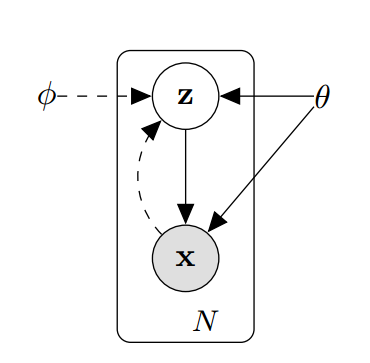
\includegraphics[height=110pt, keepaspectratio = true]{images/model}   
  \end{figure}
  \tiny \textcolor{gray} {http://arxiv.org/pdf/1312.6114v10.pdf}
\end{frame}

% 3
\begin{frame}[fragile]{Practical notes}
	\textcolor{darkred}{Problems}: 
	\begin{enumerate}
	  \item Intractable posterior $p_{\theta}(z|x) = \frac{p_{\theta}(x|z) p_{\theta}(z)}{p_{\theta(x)}}$\\
	  \item Intractable marginal likelihood $p_{\theta}(x) = \int {p_{\theta}(z) p_{\theta}(x|z) dz}$
	  \item Integrals for any reasonable mean-field VB algorithm are intractable
	  \item Large dataset, so batch optimization is too costly
  \end{enumerate}	 
	~\\
\end{frame}

% 4
\begin{frame}[fragile]{Goals}
  \begin{enumerate}
    \item Efficient approximate ML or MAP estimation for the parameters $\theta$
    \item Efficient approximate posterior inference of the latent variable $z$ given an observed value $x$
for a choice of parameters $theta$
    \item Efficient approximate marginal inference of the variable $x$ 
  \end{enumerate}
\end{frame}

%5
\begin{frame}[fragile]{Variational inference}
  Introduce parametric model $q_{\phi}(z|x)$ with variational parameters $\phi$\\
  ~\\
  \textcolor{darkred}{Idea}: Construct estimator of the variational lower bound which we can optimize jointly 
  w.r.t. $\phi$ and $\theta$\\
  ~\\
  Pro:
  \begin{itemize}
    \item Stochastic optimization
    \item Convergence
  \end{itemize}
  
\end{frame}

% 6
\begin{frame}[fragile]{Variational lower bound}
	\begin{align*} 
		\log {p_\theta (x)} &= \log \int {p_\theta (x|z) p_\theta(z) dz} \\
		&= \log \int{ \frac{q_\phi (z|x)}{q_\phi (z|x)} p_\theta (x|z) p_{\theta}(z) dz} \\
		&\ge -\mathbb{D}_{KL}[q_\phi (z|x) \parallel p_{\theta}(z)] + \mathbb{E}_{q_{\phi}} [\log p_\theta (x|z)]
	\end{align*} 

  \begin{itemize}
    \item $q(z|x)$ is not necessarily factorial
    \item Parameters $\phi$ are not computed from some closed-form expectation
  \end{itemize}

% \tiny \textcolor{gray}{Used Jensen's inequality}

\end{frame}

% 7
\begin{frame}[fragile]{Mean field}
  todo 
  % в явном виде нам q(z ) не нужна
\end{frame}

% 8
\begin{frame}[fragile]{AEVB}
  % везде нейросети
  % переход к minibatch
todo
\end{frame}

% 9
\begin{frame}[fragile]{Standart Monte-Carlo ELBO}
%  \textcolor{darkred}{Problem}: Efficient computation of $\nabla_{\phi} \mathbb{E}_{q_{\phi}} [\log p_\theta (x|z)] $\\
%  ~\\
  $\nabla_{\phi} \mathbb{E}_{q_{\phi}} [f(z)] = \mathbb{E}_{q_{\phi}(z)} \left[ f(z) \nabla_{\phi} 
  \log q_{\phi}(z) \right] \simeq \frac{1}{L} \sum\limits_{l=1}^L f(z) \nabla_{\phi} \log q_{\phi}(z^{(l)})$\\
  ~\\
  where $z^{(l)} \sim q_{\phi}(z|x)$\\
  ~\\
  \textcolor{darkred}{Problem}: Exhibits high variance
\end{frame}

% 10
\begin{frame}[fragile]{Reparametrization trick}
  \textcolor{darkred}{Idea}: Alternative method for generating samples from $q_{\phi}(z|x)$
  ~\\
  \begin{enumerate}
    \item $z \sim q_{\phi}(z|x)~-$ conditional distribution    
    \item Express $z$ as deterministic variable $z = g_{\phi}(\varepsilon, x)$\\
      where $\varepsilon$ is an auxiliary variable. $\varepsilon \sim p(\varepsilon)$
  \end{enumerate}
~\\
  $\mathbb{E}_{q_{\phi}}[f(z)] = \mathbb{E}_{p_{\varepsilon}} \left[ f(g_{\phi}(\varepsilon, x)) \right] \simeq 
  \frac{1}{L} \sum\limits_{l=1}^L f(g_{\phi}(\varepsilon^{(l)}, x))$
\end{frame}

% 11
\begin{frame}[fragile]{Reparametrization trick. Gaussian case}
  \begin{enumerate}    
    \item $q_\phi(z|x) = \mathcal{N}(z; \mu, \sigma^2)$
    \item $z = \mu + \sigma\varepsilon$ ~~ where $\varepsilon \sim \mathcal{N}(0, 1)$ 
  \end{enumerate}
  ~\\
  $\nabla_{\phi} \mathbb{E}_{q_{\phi}(z)} [f_{\theta}(z)] \Leftrightarrow 
  \mathbb{E}_{\mathcal{N}(\varepsilon| 0, 1)} [\nabla_{\phi} f_{\theta} (\mu + \sigma \varepsilon)]$
\end{frame}

% 12
\begin{frame}[fragile]{Algorithm}
  \begin{algorithmic}
    \State $\theta, \phi \gets$ initialize parameters
    \Repeat 
       \State $X^M \gets$ Random minibatch of $M$ datapoints 
       \State $\varepsilon \gets$ Random samples from noise distribution $p(\varepsilon)$
       \State $g \gets \nabla_{\phi, \theta} \mathcal{L}^M(\theta, \phi; X^M, \varepsilon) $ Gradients of minibatch estimator
       \State $\theta, \phi \gets$ Update parameters using gradients $g$
    \Until {convergence of parameters $\theta$, $\phi$}\\
    \Return $\theta$, $\phi$
  \end{algorithmic}
  
\end{frame}

% 13
\begin{frame}[fragile]{VAE inference model}
  \textcolor{darkred}{The VAE approach}: introduce an inference model that
  learns to approximate the intractable posterior by optimizing the variational lower bound: 
  $$ \mathcal{L}(\theta, \phi, x) = -\mathbb{D}_{KL}[q_{\phi} (z|x) \parallel p(z)] + 
  \mathbb{E}_q [\log p_\theta (x|z)] $$
  We parameterize with another neural network:
  \begin{figure}[htbp]
    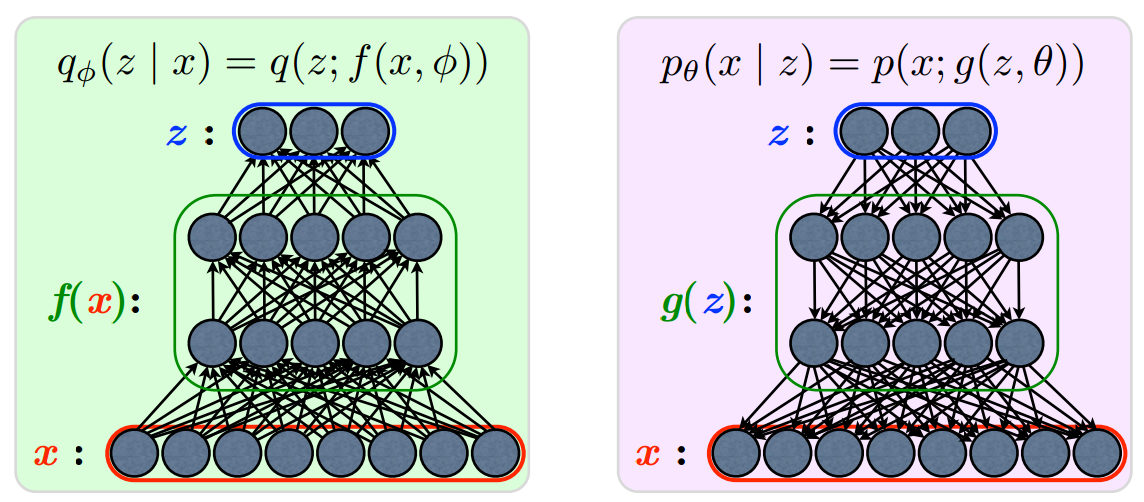
\includegraphics[height=130pt, keepaspectratio = true]{images/vae}   
  \end{figure}
  \tiny \textcolor{gray}{http://videolectures.net/deeplearning2015\_courville\_autoencoder\_extension}
\end{frame}

% 14
\begin{frame}[fragile]{Coding theory perspective}
  The unobserved variables $z$ have an interpretation as a latent representation or code.

  \begin{itemize}
    \item Represent recognition model $q_{\phi}(z|x)$ as a probabilistic encoder.\\
        Given a datapoint $x$ it produces a distribution over the possible values of the code $z$ 
        from which the datapoint $x$ could have been generated
    \item Represent $p_{\theta}(x|z)$ as a probabilistic decoder.\\
        Given a code $z$ it produces a distribution over the possible corresponding values of $x$
  \end{itemize}
\end{frame}

% 15
\begin{frame}[fragile]{Variational Auto-Encoder}
todo 
% см статью п.3
\end{frame}

% 16
\begin{frame}[fragile]{Model restriction}
  Diagonal covariance\\
  ~\\
  What can be done?\\
  ~\\
  How can we get closer to $p_{\theta}(z|x)$?
\end{frame}

% 17
\begin{frame}[fragile]{Normalizing flows}
  \textcolor{darkred}{Normalizing flows}: the transformation of a probability density through 
  a sequence of invertible mappings.
  \begin{itemize}
    \item By repeated application of the rule for random variable transformations, the initial 
    density flows through the sequence of invertible mappings.
    \item At the end of the sequence, we have a valid probability distribution.
  \end{itemize}

\end{frame}

% 18
\begin{frame}[fragile]{Normalizing flows}
  Transformation of random variables: $z' = f(z)$, $f^{-1}(z') = z$\\
  $$q(z') = q(z) \left\vert \det \frac{\partial f^{-1}(z')}{\partial z'} \right\vert = 
  q(z) \left\vert \det \frac{\partial f(z')}{\partial z'} \right\vert^{-1}$$\\
  Chaining together a sequence: $z_K = f_K \circ f_{K−1} \circ \cdots \circ f_2 \circ f_1(z_0)$\\
  $$\log q_K(z_K) = \log q_0(z_0) − \sum_{k=1}^K \log \left\vert \det \frac{\partial f_k}{\partial z_k} \right\vert $$

  Law of the unconscious statistician:\\
  $$\mathbb{E}_{q_K} \left[g(z_K)\right] = \mathbb{E}_{q_0} \left[ g(f_K \circ f_{K−1} \circ \cdots \circ f_2 
  \circ f_1(z_0)) \right] $$
\end{frame}

% 19
\begin{frame}[fragile]{Planar flow}
  Family of transformations: $f(z) = z + uh\left( w^T z + b \right)$\\
  ~\\
  $$\left\vert \det \frac{\partial f(z)}{\partial z} \right\vert = \left\vert 1 + u^T \psi(z) 
  \right\vert ~~~\text{where}~~~ \psi(z) = h'(w^Tz + b)w$$ \\
  $$\log q_K(z_K) = \log q_0(z_0) − \sum_{k=1}^K \log \left\vert 1 + u^T \psi(z) \right\vert $$
  % картиночки (применение потока + обучение потока)
  %геометрический смысл
\end{frame}

% 20
\begin{frame}[fragile]{Radial flow}
  todo
\end{frame}

% 21
\begin{frame}[fragile]{Examples}
  todo
  % картинка про поток?
\end{frame}

% 22
\begin{frame}[fragile]{Variational lower bound}
  \begin{align*} 
  \mathcal{L}(\theta, \phi, x) &= \mathbb{E}_{q_\phi(z|x)} \left[ \log p_\theta(x, z) - \log q_\phi(z | x) \right] \\
  &= \mathbb{E}_{q_K(z_K)} \left[ \log p(x, z_K) - \log q(z_K) \right] \\
  &= \mathbb{E}_{q_0(z_0)} \left[ \log p(x, z_K) - \log q_0(z_0) + \sum_{k=1}^K \log \left\vert \det 
  \frac{\partial f_k}  {\partial z_k} \right\vert \right] 
  \end{align*} 
\end{frame}

% 23
\begin{frame}[fragile]{Algorithm}
  \begin{algorithmic}
    \State $\theta, \phi \gets$ initialize parameters
    \Repeat 
       \State $X^M \gets$ Random minibatch of $M$ datapoints 
       \State $\varepsilon \gets$ Random samples from noise distribution $p(\varepsilon)$
       \State $g \gets \nabla_{\phi, \theta} \mathcal{L}^M(\theta, \phi; X^M, \varepsilon) $ Gradients of minibatch estimator
       \State $\theta, \phi \gets$ Update parameters using gradients $g$
    \Until {convergence of parameters $\theta$, $\phi$}\\
    \Return $\theta$, $\phi$
  \end{algorithmic}
  
\end{frame}

% 24
\begin{frame}[fragile]{MNIST (vae, vae+nf)}
  todo
  %картинки
  % график ELBO
\end{frame}

% 25
\begin{frame}[fragile]{лица?}
  todo
  %картинки
\end{frame}

% 26
\begin{frame}[fragile]{Future experiments}
  todo 
\end{frame}

\end{document}
